\section{Convex Optimization Problems}

Recall general optimization Problem
\begin{equation}
	\begin{aligned}
		\operatorname{minimize}\quad & f(x)                               \\
		\text{s.t.}                  & g_i(x) \le 0,\quad i = 1,\dots,n_g \\
		                             & h_i(x) = 0,\quad i = 1,\dots,n_h   \\
	\end{aligned}
	\label{eq:optimization}
\end{equation}

OPTIMAL VALUE

\subsection{Feasibility  Problem}

\begin{equation}
	\begin{aligned}
		\operatorname{minimize}\quad & s                                  \\
		\text{s.t.}                  & g_i(x) \le s,\quad i = 1,\dots,n_g \\
		                             & h_i(x) = 0,\quad i = 1,\dots,n_h   \\
	\end{aligned}
\end{equation}

\subsection{Linear Programming}

\begin{equation}
	\begin{aligned}
		\operatorname{minimize}\  & c\T x & \text{s.t.}\  & Ax-b \ge 0,\ x\ge0
	\end{aligned}
\end{equation}

Derive dual problem:

Step 1: $\mathcal{L}(x,\lambda_1,\lambda_2) = c\T x-\lambda_1\T (Ax-b) -\lambda_2\T x,\ \lambda_i \ge0$

Step 2:$\underset{x \in \mathcal{\mathbb{R}}^n}{inf}\mathcal{L}(x,\lambda_1,\lambda_2)
	= \begin{cases} \lambda_1\T b & \text{if }c-A\T\lambda_1-\lambda_2=0  \\
              -\infty       & \text{if } c-A\T\lambda_1-\lambda_2=0\end{cases}$

Step 3: Dual Problem (again linear programm)
\begin{equation}
	\begin{aligned}
		\operatorname{maximize}\  & b\T\lambda & \text{s.t.}\  & c-A\T\lambda \ge 0,\ \lambda\ge0
	\end{aligned}
\end{equation}

\subsubsection{Skech}

- Polyhedron

- c-vector normal gives 'Levelsets'

- Optimal solution in or trough a corner (if exists)

\begin{proposition}
	The optimal solution of a linear program (if it exists)
	lies always on the boundary of the feasible set
	and there exists an optimal solution that is a vertex of the feasible set.
\end{proposition}

\subsubsection{Shortest Path}

Analogie with Fluid

Soltuion greater 0, not optimal edges = 0

\subsection{Quadratic Programming}

minimmize $\frac{1}{2}x\T Px+q\T x$
s.t. $Gx\le h,\ Ax=b$

Interpretation: minimize a convex quadratic function over a polyhedron.

If $P=P\T$ is positive semi-definite
then the problem is convex.

\textbf{Example} [optimal control] (basis for mpc)
%todo

\subsubsection{Second-order cone program (SOCP)}

minimmize $f\T x$

s.t. $|A_ix+b|\le c_i\T x+d_i,\ Fx=g$

Second-order cone
$C_{n+1}=\{ (x,t)\mid
	x\in\mathbb{R}^{n}, t\in \mathbb{R}, |x|\le t \}$

\textbf{Example} [Markovitz portfolio optimization:]

\begin{itemize}
	\item $n$ number of assets/stocks
	\item $x_i$ relative value of asset $i$
	\item $p_i$ price change of stock $i$
	\item $p^Tx$ overall return
\end{itemize}

Constraints

\begin{itemize}
	\item $x^T\textbf{1} = B$, total amount
	\item $x\ge0$, no short position
\end{itemize}

CALCULATIONS

\subsection{Semidefinite programming (SDP)}

minimmize $c\T x$

s.t. $x_1F_1,\dots+x_nF_n <= 0$ and $Ax-b=b$

$\rightarrow$ the 'standard' form

$$\min _{x \in \mathbb{R}^{n*n}} tr(CX)$$

Problem Classes

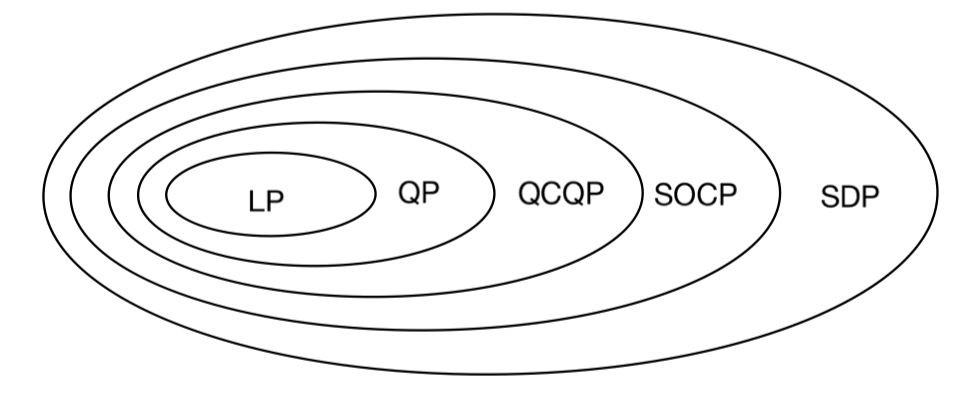
\includegraphics[width=\columnwidth]{images/problem_class.png}
